\chapter{Marketing}\label{ch:marketing}

Marketing je všeude kolem nás. Týká se nás více či méně, ať už si to uvědomujeme, nebo ne. V této kapitole uvedeme pojem \textbf{marketing} a seznámíme se s jeho účelem, hodnotami a procesem.

\section{Účel marketingu}

Jedna z nejstručnějších definic marketingu říká, že \textbf{marketing} je o naplňování potřeb se ziskem.\cite{kotler2007marketingmanagement} Marketing tak činí komplexní řadou aktivit, které zahrnují tvorbu výrobků a služeb, podporu jejich existence a vlastností a jejich fyzického zpřístupnění cílovým uživatelům -- distribuce.\cite{clemente2004slovnikmarketingu}
Tyto aktivity jsou známé jako tzv. \textbf{\uv{4P marketingu}} nebo také \textbf{\uv{merketingový mix}} (viz dále).

V zásadě můžeme také rozlišovat mezi \textbf{společenskou} a \textbf{manažerskou} definicí marketingu. Společenská definice chápe marketing jako společenský proces, ve kterém jsou hlavními aktéry jedinci a skupiny, kteří svobodně směňují, tj. nabízí a kupují, výrobky a služby. Manažerská definice naopak dosazuje za hlavního aktéra samotného prodejce a označuje marketing jako "umění prodeje výrobků"\cite{kotler2007marketingmanagement}.
Prodej výrobků jistě uměním je, nicméně může být pro některé překvapením, že nejdůležitější částí marketingu není prodej!

Jak uvádí Peter Drucker, přední teoretik managementu\cite{kotler2007marketingmanagement}:
\begin{aquote}{Peter Drucker}
\uv{Lze předpokládat, že vždy bude existovat potřeba něco prodávat. Cílem marketingu je však učinit prodávání čímsi nadbytečným. Cílem marketingu je poznat a pochopit zákazníka natolik dobře, aby mu výrobek, nebo služba padly jako šité na míru a prodávaly se samy. V ideálním případě by měl marketing vyústit v získání zákazníka ochotného nakupovat. Vše, čeho je pak zapotřebí, je učinit výrobek, či službu dostupnými.}
\end{aquote}

\section{4P marketingu}

Pojem \uv{marketingový mix}, známý také jako tzv. \uv{4P marketingu}, začal používat ve svých projevech prof. Neihl H. Borden a definoval jej v jedné ze svých publikací\cite{borden1964marketingmix} v roce 1949. V publikaci Borden říká, že tento pojem mu vnukl jeho spolupracovník -- prof. James Culliton. Ve své studii z roku 1948 Culliton definoval výkoného manažera jako umělce, který \uv{míchá ingredience} a který se \uv{někdy řídí receptem připraveným ostatními, jindy vymýšlí svůj vlastní. Někdy přihodí do receptu ingredienci, které je zrovna dostupná a jindy experimentuje s ingrediencemi, které nikdo nikdy nezkoušel.}

Marketingový mix tvoří čtyři kontrolovatelné proměnné, které společnost reguluje, aby efektivně prodávala výrobek. Jedná se o proměnné: \textbf{výrobek}, \textbf{cena}, \textbf{místo} a \textbf{reklama} (z anglického \textit{product}, \textit{price}, \textit{place}, \textit{promotion})\cite{clemente2004slovnikmarketingu}.
S nadsázkou lze o marketingu prohlásit, že se jedná pouze o to postavit správný produkt na správné místo za správnou cenu ve správný čas. Možná proto také hovoříme o marketingu jako o vědě --- je potřeba udělat spoustu věcí správně.


\subsection{Výrobek}
    
Výrobek je definován jako entita mající objektivní a subjektivní charakteristiky, které jsou manipulovány k maximu jeho přitažlivosti pro cílové zákazníky\cite{clemente2004slovnikmarketingu}. Výrobkem je tedy v podstatě jakékoli \textit{průmyslové} či \textit{spotřební zboží} vytvořené za účelem zisku.
Průmyslové zboží je zboží určeno primárně pro výrobu dalších výrobků. Patří sem například suroviny, zařízení nebo zpracovatelské materiály.
Spotřební zboží pak lze dále dělit na zboží \textit{dlouhodobé} a \textit{krátkodobé spotřeby} a \textit{balené} zboží.


\subsection{Cena}
Cena je jediným prvkem marketingového mixu, který společnosti \textbf{generuje výnosy}. Vztahuje se k stanovení nákladů na výrobek k maximálnímu prodeji a zvýšení image výrobku. Cena má nezanedbatelný vliv na představu spotřebitele o výrobku\cite{clemente2004slovnikmarketingu}.


\subsection{Místo}
Každý výrobek je potřeba někde skladovat a nějakým způsobem distribuovat (distribuce se týká i služeb) spotřebitelům. K tomu je potřeba vhodná \textit{taktika} a \textit{distribuční kanály}. Distribuce pak může být jak fyzického charakteru -- skladování a přeprava, tak virtuálně (např. zakoupení poukazu či subskripce). Kanály dělíme obecně na \textit{přímé} a \textit{nepřímé}:

\begin{itemize}
    \item přímé kanály -- zahrnují prodej přímo spotřebitelům
    \item nepřímé kanály -- spoléhají se na maloobchodníky, velkoobchodníky a jiné zprostředkovatele\footnote{Ačkoli je tato metoda dražší, společnosti mohou dosáhnout více zákazníků pomocí nepřímých kanálů, než pomocí ostatních distribučních postupů\cite["marketingový mix", s. 114]{clemente2004slovnikmarketingu}}
\end{itemize}

Speciální kombinací přímých a nepřímých kanálů pak vznikají tzv. \textit{mnohonásobné kanály}. Pracovníci marketingu si pak ale musí být vědomi potenciálními rivaly mezi kanály.


\subsection{Reklama}
Slovník marketingu definuje reklamu jako \uv{Marketingové a komunikační taktiky používané k uvědomování cílových spotřebitelů o charakteristikách, přínosech a dostupnosti výrobku.}\cite["reklama", s. 115]{clemente2004slovnikmarketingu} Obyčejně reklama samotná není jedinou formou propagace produktu. Dalšími způsoby může být osobní prodej a publicita nebo P.R (z anglického \uv{\textit{public relations}}).


\section{Vývoj marketingu}

I pro člověka neznalého marketingové teorie není příliš obtížně pozorovat změny na trhu\footnote{V tomto kontextu myšleno jako trh spotřebitele, tj. skupiny potenciálních kupujících}.
Za hlavní \uv{viníky} těchto změn lze označit dva faktory, které měly (a mají) majoritní dopad na vývoj ekonomiky a rovněž marketingu -- \textbf{technologie} a s ní související \textbf{globalizace}. Kotler ve své knize \textit{Chaotika}\cite[s. 14]{kotler2009chaotika} uvádí:

\begin{aquote}{zdroj: \textit{Chaotika}}
\uv{Svět je propojenější a vzájemně závislejší než kdykoli předtím. Globalizace a technologie jsou dvěma hlavními silami, které vedly k vytvoření provázané křehkosti ve světové ekonomice.}
\end{aquote}

V novém informačním věku je produkční úroveň přesnější, reklama cílenější a nabídka personalizovaná. Dostupnost zboží je technologickým pokrokem v dopravě a komunikaci prakticky neomezená a v mnoha případech téměř okamžitá. Internet se stává \textbf{novým prodejním kanálem}. Díky rostoucí otevřenosti a dostupnosti internetu jsou spotřebitelé informovanější, porovnání výrobků desítek dodavatelů je dnes otázkou několika kliknutí a portály se plní uživatelskými recenzemi, ať už pozitivními, či nikoli.
Moderní spotřebitelé hodnotí značku podle toho, jak moc se o ní mluví, jak moc je autentická a jedinečná a jaké v emoce značka vyvolává. Chtějí se se značkou \textit{ztotožnit}.\cite{bergh2012coolznacky}
Tyto a další důvody vedou také k přesunu moci do rukou zákazníků --- slovní spojení \uv{náš zákazník, náš pán} tak v posledních letech dosahuje dosud nevídaných rozměrů --- a zákazníci tak očekávají stále lepší služby, vyšší kvalitu a pohodlí a individuální přístup.

\subsection{Holistický marketing}

Společnosti tak potřebují nový způsob myšlení o tom, jak působit a soupeřit v novém marketingovém prostředí. Touto novou koncepcí je tzv. \textit{holistický merketing}.
\uv{\textbf{Holistické marketingové pojetí} je postaveno na vývoji, designu a plnění marketingových programů, procesů a aktivit beroucích v úvahu jejich šíři a vzájemnou propojenost.}\cite{kotler2007marketingmanagement} Holistický marketing zavádí novou perspektivu, ve které \textbf{záleží na všem}. Jeho složky jsou shrnuty na obr. \ref{fig:slozky-holistickeho-marketingu}.

\begin{figure}[htbp!]
    \centering
    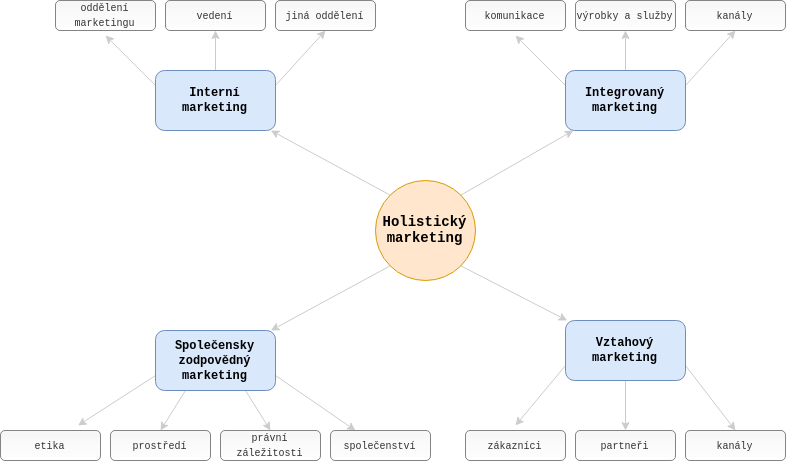
\includegraphics[width=.88\textwidth]{assets/slozky-holistickeho-marketingu.png}
    \caption[Složky holistického marketingu]{Složky holistického marketingu \\ Zdroj: Vlastní zpracování dle \textcite[s. 56]{kotler2007marketingmanagement}}
    \label{fig:slozky-holistickeho-marketingu}
\end{figure}

Je potřeba si uvědomit (a částečně se tak i uklidnit), že informační kvanta nejsou užitečná pouze a jen pro cílové spotřebitele, ale lze je s výhodou použít také pro marketingové účely.